\setcounter{section}{4}
\setlength{\parindent}{0pt}  % nessun rientro
\setlength{\parskip}{6pt}    % spazio tra paragrafi

\section{Use Case Diagram}

Questa sezione descrive i principali casi d’uso del sistema \textbf{Rinova}, suddivisi per categoria di attore. 
Per ogni gruppo funzionale viene riportato il relativo \textit{Use Case Diagram (UCD)} e la descrizione testuale 
dei singoli requisiti funzionali (\textit{RF}) con riassunto, flusso principale ed eventuali eccezioni.

% =========================================================
\subsection*{Use Case Diagram – Requisiti funzionali comuni}
% =========================================================

\subsubsection*{UCD-01 – Registrazione e login utente}
\begin{itemize}
    \item RF-01 – Registrazione utente
    \item RF-02 – Login utente
    \item RF-02.1 – Recupero password
\end{itemize}

\begin{figure}[H]
    \centering
    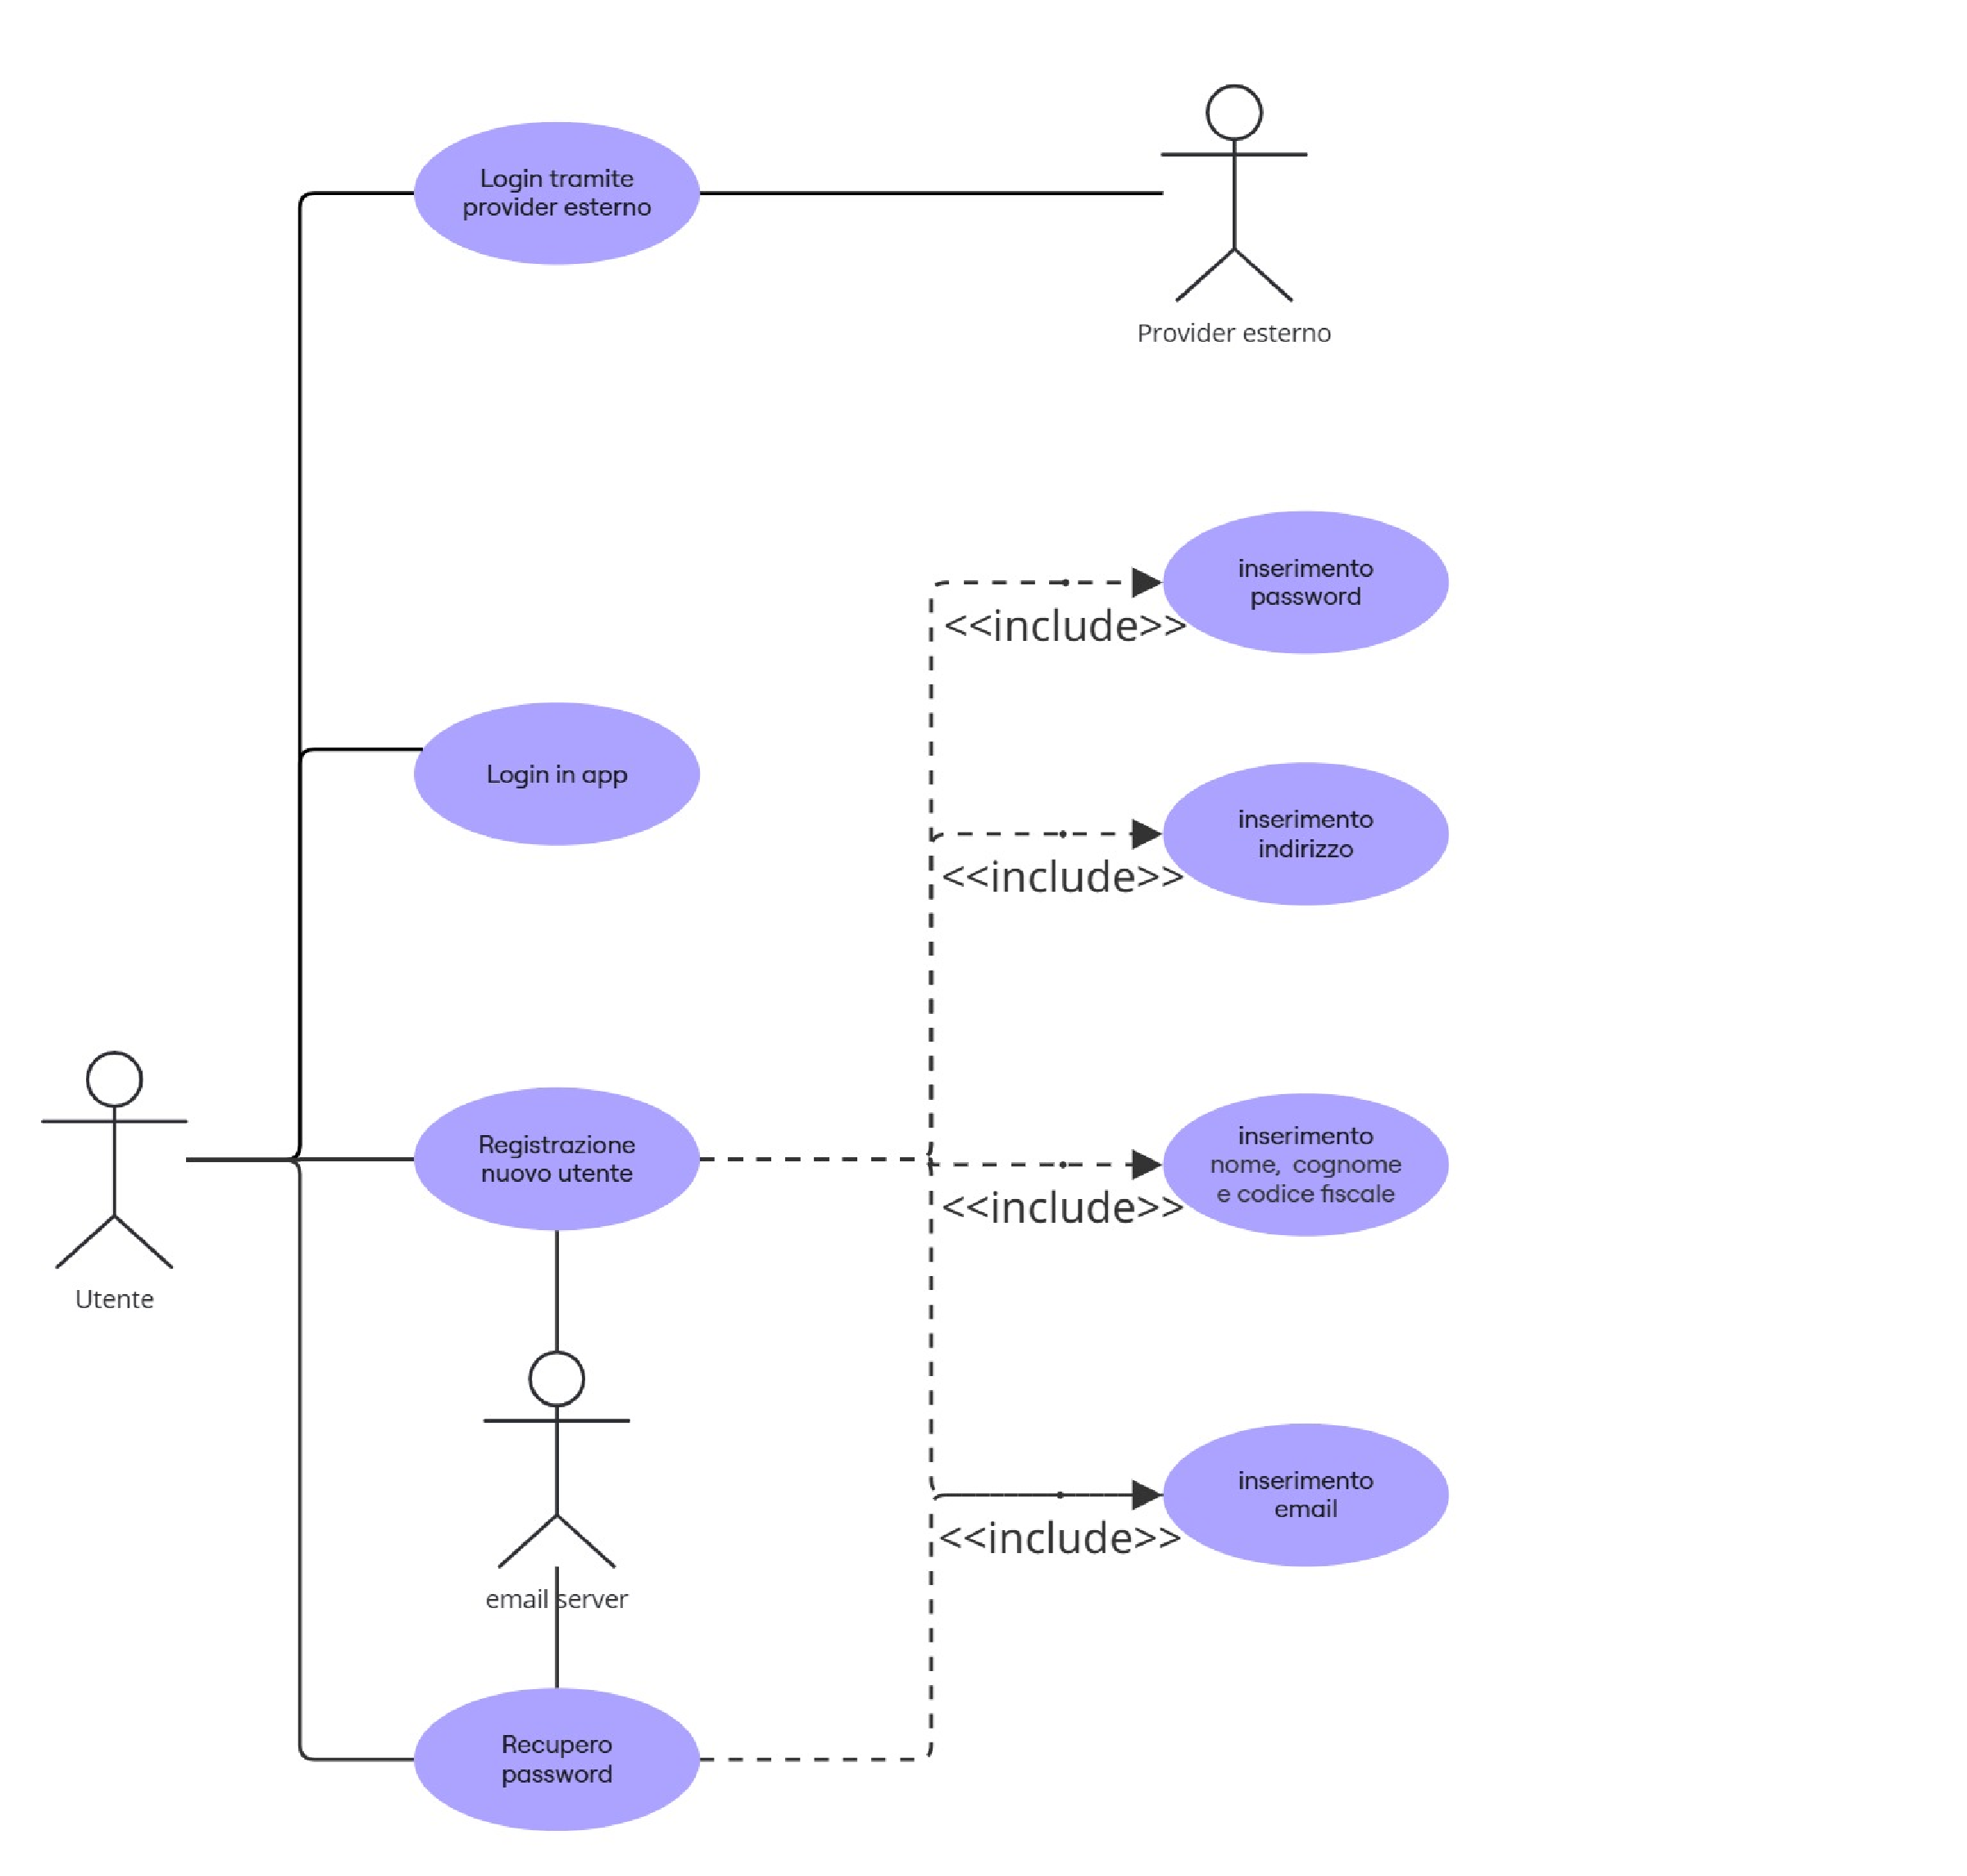
\includegraphics[width=0.9\textwidth]{images/use_case/ucd_01.pdf}
    \caption{UCD-01 – Registrazione e login utente}
    \label{fig:ucd01}
\end{figure}

% ------------------------
\paragraph*{Use Case RF-01: Registrazione utente}
\subparagraph*{Riassunto:}
Questo use case descrive come l'utente anonimo effettua la prima registrazione alla webapp.

\subparagraph*{Descrizione:}
\begin{enumerate}
    \item L’utente anonimo visualizza la schermata di registrazione con il form contenente i campi obbligatori: Nome, Cognome, Email, Codice fiscale, Numero di telefono, Comune di residenza e Password.
    \item L’utente compila i campi obbligatori e, opzionalmente, quelli non obbligatori; quindi preme il pulsante ``Registrati''.
    \item L'utente accetta i termini e condizioni per la privacy.
    \item Il sistema valida i dati inseriti (campi obbligatori, formato di nome/cognome, formato email, unicità email e codice fiscale, formato numero di telefono, criteri password).
    \item Se la validazione ha esito positivo, il sistema crea il profilo utente e invia una email di conferma contenente un link di verifica e/o una password temporanea.
    \item L’utente clicca il link nella email per confermare l’indirizzo; il sistema finalizza la registrazione e imposta lo stato account a ``attivo'' (o ``in attesa'' se è previsto controllo manuale).
\end{enumerate}

\subparagraph*{Eccezioni:}
\begin{itemize}
    \item Se mancano campi obbligatori, il sistema segnala gli errori e impedisce la registrazione.
    \item Se email o codice fiscale sono già registrati, il sistema notifica la collisione e richiede correzione.
    \item Se il formato della password non soddisfa i criteri, il sistema richiede una password conforme.
\end{itemize}

% ------------------------
\paragraph*{Use Case RF-02: Login utente}
\subparagraph*{Riassunto:}
Questo use case descrive come l'utente autenticato effettua il login nella webapp.

\subparagraph*{Descrizione:}
\begin{enumerate}
    \item L’utente visualizza la schermata di login con campi Email/Username e Password e opzioni di autenticazione esterna (Google, Microsoft).
    \item L’utente inserisce Email e Password e preme ``Accedi''.
    \item Il sistema verifica le credenziali: se corrette reindirizza l’utente alla homepage personalizzata; in caso contrario mostra errore.
    \item Se l’utente seleziona un provider OAuth2 (es. Google), viene reindirizzato alle schermate del provider; dopo autenticazione corretta il sistema accetta il token e apre la homepage.
\end{enumerate}

\subparagraph*{Eccezioni:}
\begin{itemize}
    \item Se email/password non corrispondono, il sistema mostra un messaggio di errore e offre il recupero password.
    \item Se l’autenticazione tramite provider esterno fallisce o è annullata, il sistema ritorna alla schermata di login e notifica l’errore.
\end{itemize}

% ------------------------
\paragraph*{Use Case RF-02.1: Recupero password}
\subparagraph*{Riassunto:}
Questo use case descrive come un utente che ha dimenticato la password richiede e completa il reset della password.

\subparagraph*{Descrizione:}
\begin{enumerate}
    \item L’utente seleziona ``Recupera password'' dalla schermata di login e inserisce il proprio indirizzo email.
    \item Il sistema verifica che l’email sia registrata e invia un’email contenente un link sicuro per il reset (con token a scadenza).
    \item L’utente clicca il link e viene reindirizzato a una pagina per inserire la nuova password.
    \item L’utente inserisce la nuova password che deve rispettare i criteri di sicurezza; il sistema aggiorna la password e conferma l’avvenuto reset.
\end{enumerate}

\subparagraph*{Eccezioni:}
\begin{itemize}
    \item Se l’email non è registrata, il sistema notifica l’utente (senza rivelare dati sensibili).
    \item Se il token è scaduto o invalido, il sistema richiede una nuova richiesta di recupero.
\end{itemize}

% =========================================================
\subsection*{UCD-02 – Accesso all'area personale, modifica dati e cancellazione account}
% =========================================================

\begin{itemize}
    \item RF-03 – Accesso all'area personale
    \item RF-03.1 – Modifica dati personali
    \item RF-03.2 – Modifica email
    \item RF-03.3 – Modifica numero di telefono
    \item RF-03.4 – Cancellazione dell'account
    \item RF-04 – Logout utente
\end{itemize}

\begin{figure}[H]
    \centering
    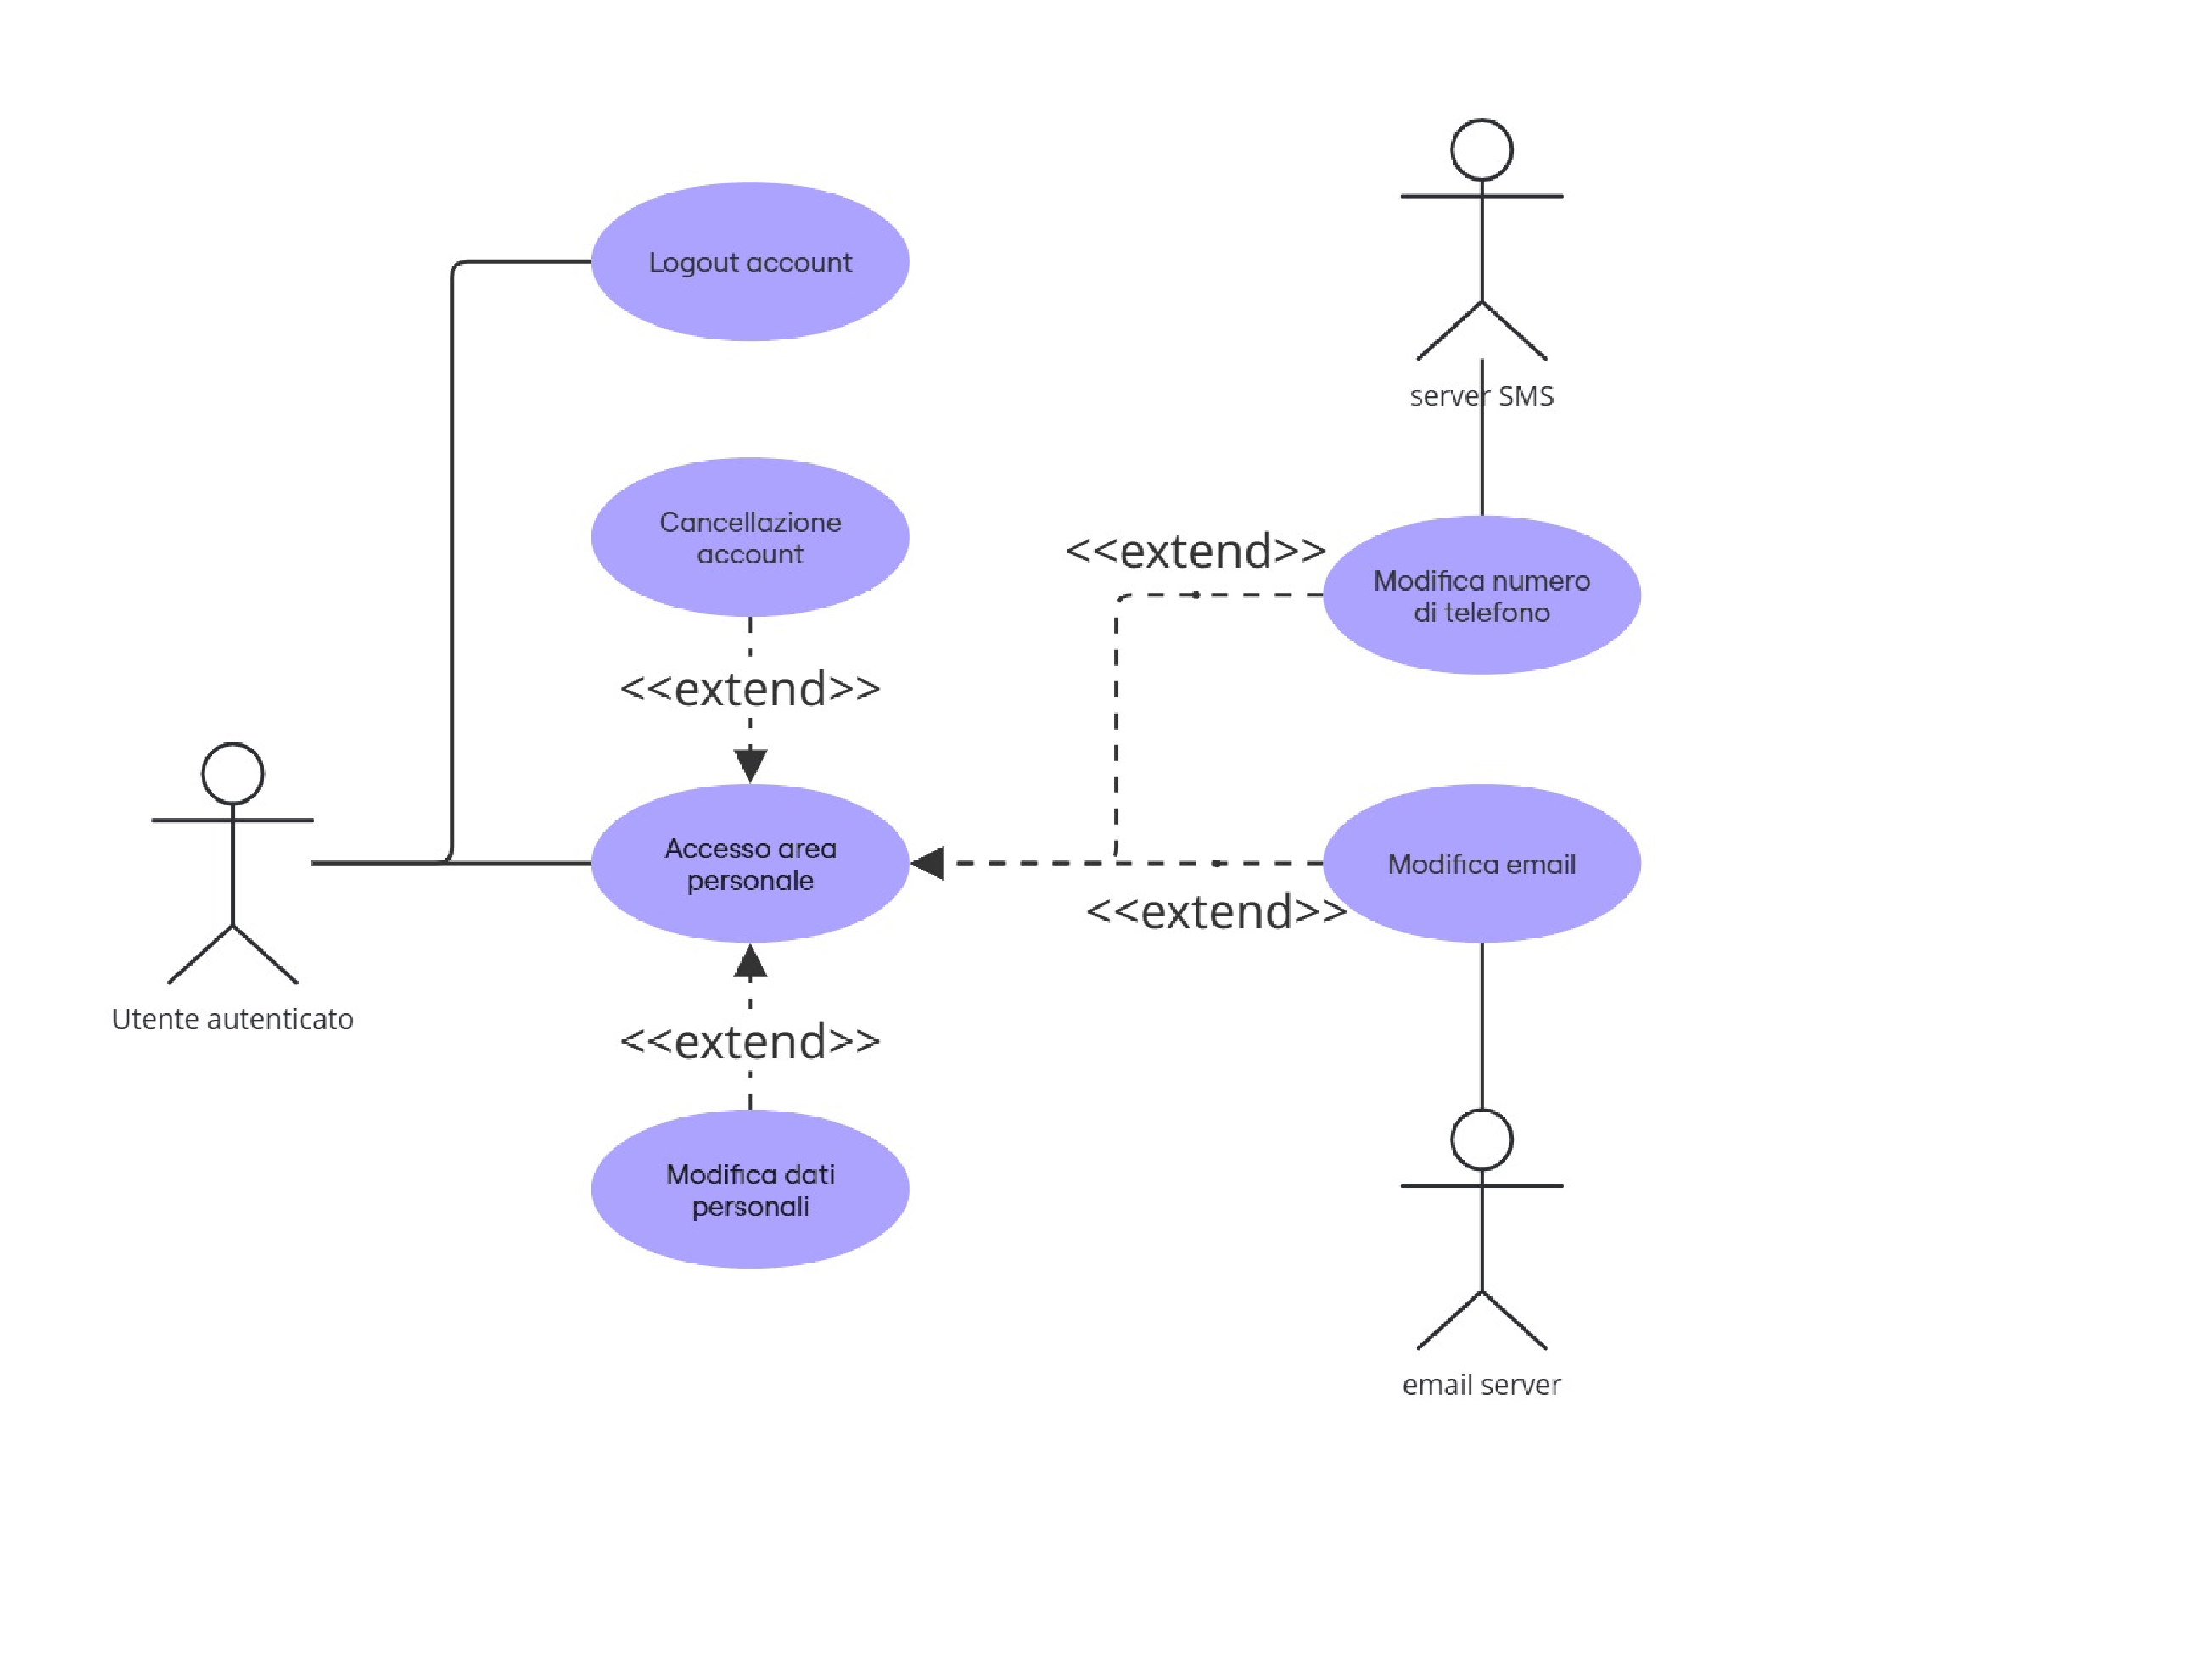
\includegraphics[width=0.9\textwidth]{images/use_case/ucd_02.pdf}
    \caption{UCD-02 – Accesso all’area personale, modifica e cancellazione account}
    \label{fig:ucd02}
\end{figure}

% ------------------------
\paragraph*{Use Case RF-03: Accesso all'area personale}
\subparagraph*{Riassunto:}
Questo use case descrive come un utente autenticato accede alla propria area personale per visualizzare il profilo e le impostazioni.

\subparagraph*{Descrizione:}
\begin{enumerate}
    \item L’utente effettua il login con successo.
    \item Dalla homepage o dalla navbar seleziona ``Area personale''.
    \item Il sistema autentica la sessione e mostra la pagina con i dati del profilo, impostazioni dell’account e le funzionalità disponibili (modifica dati, notifiche, gestione privacy).
    \item L’utente può navigare le sotto-sezioni per modificare informazioni o avviare operazioni (es. cancellazione account).
\end{enumerate}

\subparagraph*{Eccezioni:}
\begin{itemize}
    \item Se la sessione è scaduta o non autenticata, il sistema reindirizza alla pagina di login.
    \item Se l’utente non ha i permessi necessari per una funzionalità, il sistema mostra un messaggio di accesso negato.
\end{itemize}

% ------------------------
\paragraph*{Use Case RF-03.1: Modifica dati personali}
\subparagraph*{Riassunto:}
Questo use case descrive come un utente modifica o elimina (se permesso) i propri dati personali dall’area personale.

\subparagraph*{Descrizione:}
\begin{enumerate}
    \item L’utente autenticato entra nell’area personale e seleziona ``Modifica profilo''.
    \item Il sistema presenta il form con i dati correnti; l’utente modifica i campi ammessi.
    \item L’utente conferma le modifiche; il sistema valida i nuovi dati e, se validi, li salva aggiornando il profilo.
    \item Il sistema registra l’operazione nel registro attività e notifica l’utente dell’avvenuta modifica.
\end{enumerate}

\subparagraph*{Eccezioni:}
\begin{itemize}
    \item Se i dati inseriti non superano la validazione (formati errati, duplicati), il sistema mostra errori e non salva.
    \item Alcuni campi obbligatori non possono essere eliminati: il sistema impedisce la rimozione e informa l’utente.
\end{itemize}

% ------------------------
\paragraph*{Use Case RF-03.2: Modifica email}
\subparagraph*{Riassunto:}
Questo use case descrive come un utente modifica l’indirizzo email associato al proprio account.

\subparagraph*{Descrizione:}
\begin{enumerate}
    \item L’utente accede all’area personale e seleziona ``Cambia email''.
    \item Inserisce il nuovo indirizzo email; il sistema verifica il formato e che non sia già in uso.
    \item Il sistema invia una email di conferma al nuovo indirizzo con un link di verifica.
    \item L’utente clicca il link: il sistema valida il token e aggiorna l’email nel profilo, eventualmente notificando il vecchio indirizzo.
\end{enumerate}

\subparagraph*{Eccezioni:}
\begin{itemize}
    \item Se il nuovo indirizzo è già registrato, il sistema blocca l’operazione e segnala l’errore.
    \item Se l’utente non conferma la mail (link non cliccato / token scaduto), la modifica non viene applicata.
\end{itemize}

% =========================================================
\paragraph*{Use Case RF-03.3: Modifica numero di telefono}
\subparagraph*{Riassunto:}
Questo use case descrive come l'utente modifica il proprio numero di telefono dall'area personale.

\subparagraph*{Descrizione:}
\begin{enumerate}
    \item L’utente seleziona ``Modifica numero di telefono'' nell’area personale.
    \item Inserisce il nuovo numero; il sistema verifica il formato internazionale e la validità di base.
    \item Il sistema può inviare un SMS con un codice OTP al nuovo numero; l’utente inserisce il codice per confermare.
    \item Se la verifica ha esito positivo, il sistema aggiorna il numero nel profilo.
\end{enumerate}

\subparagraph*{Eccezioni:}
\begin{itemize}
    \item Se il formato del numero è errato, il sistema segnala l’errore.
    \item Se l’OTP non è corretto o scade, la modifica non viene applicata.
\end{itemize}

% =========================================================
\paragraph*{Use Case RF-03.4: Cancellazione dell'account}
\subparagraph*{Riassunto:}
Questo use case descrive come l'utente può richiedere la cancellazione permanente del proprio account.

\subparagraph*{Descrizione:}
\begin{enumerate}
    \item L’utente autenticato apre l’area personale e seleziona ``Elimina account''.
    \item Il sistema mostra un avviso con informazioni sulle conseguenze e chiede conferma esplicita (inserire la password).
    \item Dopo la conferma, il sistema avvia il processo di cancellazione: rimuove i dati personali in conformità con le normative e aggiorna lo stato account a ``cancellato''.
\end{enumerate}

\subparagraph*{Eccezioni:}
\begin{itemize}
    \item Se l’utente non fornisce conferma esplicita, la cancellazione non procede.
    \item Se esistono vincoli legali o dati che devono essere conservati (es. obblighi normativi), il sistema informa l’utente e non cancella tali dati; esegue invece l’anonimizzazione quando possibile.
\end{itemize}

% =========================================================
\paragraph*{Use Case RF-04: Logout utente}
\subparagraph*{Riassunto:}
Questo use case descrive come un utente autenticato esegue il logout dalla webapp per terminare la propria sessione e garantire la sicurezza del proprio account.

\subparagraph*{Descrizione:}
\begin{enumerate}
    \item L’utente autenticato, dalla barra di navigazione o dal menù dell’area personale, seleziona l’opzione ``Logout''.
    \item Il sistema invalida la sessione corrente, eliminando eventuali token di autenticazione locali e di sessione (cookie o JWT).
    \item Il sistema reindirizza l’utente alla homepage pubblica o alla schermata di login.
    \item L’utente non ha più accesso alle funzionalità riservate fino a un nuovo login.
\end{enumerate}

\subparagraph*{Eccezioni:}
\begin{itemize}
    \item Se la sessione è già scaduta, il sistema mostra un messaggio informativo e reindirizza comunque alla homepage pubblica.
    \item Se si verifica un errore nella disconnessione (es. token non trovato o già invalido), il sistema elimina comunque i dati locali e forza il logout.
\end{itemize}


% =========================================================
\subsection*{Use Case Diagram – Requisiti funzionali per Admin della CER}
% =========================================================

\subsubsection*{UCD-03 – Gestione e approvazione membri della CER}
\begin{itemize}
    \item RF-05 – Gestione membri della CER
    \item RF-06 – Approvazione richieste di adesione
\end{itemize}

\begin{figure}[H]
    \centering
    
\includegraphics[width=0.9\textwidth]{images/use_case/ucd_03.pdf}
    \caption{UCD-03 – Gestione e approvazione membri della CER}
    \label{fig:ucd03}
\end{figure}

% ------------------------
\paragraph*{Use Case RF-05: Gestione membri della CER (Admin)}
\subparagraph*{Riassunto:}
Questo use case descrive come l’amministratore della CER gestisce l’elenco dei membri (visualizza, aggiunge, modifica, rimuove).

\subparagraph*{Descrizione:}
\begin{enumerate}
    \item L’amministratore effettua login con privilegi admin e accede al pannello di gestione membri.
    \item Il sistema mostra la lista dei membri con dati identificativi, punti di consumo/produzione e stato di partecipazione.
    \item L’amministratore può invitare un nuovo membro selezionando il pulsante ``invita membro'' ed inserendo i dati richiesti; il sistema li verifica e invia l'invito.
    \item L’amministratore può selezionare un membro per modificarne i dati o rimuoverlo attraverso l'opzione ``rimuovi membro''; tutte le operazioni sono tracciate nel registro attività.
\end{enumerate}

\subparagraph*{Eccezioni:}
\begin{itemize}
    \item Se i dati inseriti non sono validi o confliggono con record esistenti, il sistema segnala l’errore.
    \item La rimozione di un membro con vincoli (es. impianti associati) può richiedere passaggi aggiuntivi (reassegnazione impianti).
\end{itemize}

% ------------------------
\paragraph*{Use Case RF-06: Approvazione richieste di adesione (Admin)}
\subparagraph*{Riassunto:}
Questo use case descrive come l’amministratore approva o rifiuta le richieste di adesione alla CER.

\subparagraph*{Descrizione:}
\begin{enumerate}
    \item L’amministratore accede all’elenco delle richieste di adesione pendenti attraverso l'apposito pulsante ``richieste in attesa'' nel pannello di gestione membri.
    \item Seleziona una richiesta per visualizzare i dettagli (dati utente, indirizzo, disponibilità impianto, codice POD).
    \item L’amministratore può ora decidere se approvare o rifiutare la richiesta premendo gli appositi pulsanti: se approva, il sistema invia una notifica email e imposta lo stato a ``membro attivo''; se rifiuta, invia notifica con motivazione.
    \item Tutte le decisioni vengono registrate nel registro attività.
\end{enumerate}

\subparagraph*{Eccezioni:}
\begin{itemize}
    \item Se mancano informazioni necessarie per la valutazione, il sistema richiede integrazione dati.
    \item In caso di conflitti (es. POD già associato), il sistema segnala la problematica e blocca l’approvazione.
\end{itemize}

% =========================================================
\subsubsection*{UCD-04 – Gestione, monitoraggio e analisi impianti energetici}
% =========================================================

\begin{itemize}
    \item RF-07 – Gestione impianti energetici
    \item RF-08 – Monitoraggio stato impianti
    \item RF-09 – Gestione dati energetici e reportistica
    \item RF-10 – Analisi dei benefici energetici ed economici
\end{itemize}

\begin{figure}[H]
    \centering
    
\includegraphics[width=0.9\textwidth]{images/use_case/ucd_04.pdf}
    \caption{UCD-04 – Gestione, monitoraggio e analisi impianti energetici}
    \label{fig:ucd04}
\end{figure}

% ------------------------
\paragraph*{Use Case RF-07: Gestione impianti energetici (Admin)}
\subparagraph*{Riassunto:}
Questo use case descrive la registrazione, associazione e gestione degli impianti produttivi di energia rinnovabile.

\subparagraph*{Descrizione:}
\begin{enumerate}
    \item L’amministratore seleziona ``Nuovo impianto'' nella sezione degli impianti della CER e compila i dati tecnici: codice identificativo, potenza nominale, posizione geografica, data di installazione, stato operativo, ecc.
    \item Il sistema valida i dati e salva l’impianto associandolo al membro indicato.
    \item L’amministratore può aggiornare i dati tecnici o sospendere/rimuovere l’impianto (per manutenzione o dismissione).
    \item Ogni modifica viene registrata nel registro delle attività.
\end{enumerate}

\subparagraph*{Eccezioni:}
\begin{itemize}
    \item Se i dati di localizzazione o identificativi sono mancanti o incongruenti, il sistema segnala l’errore.
    \item La rimozione di un impianto con dati storici potrebbe richiedere conservazione dei dati o esportazione.
\end{itemize}

% ------------------------
\paragraph*{Use Case RF-08: Monitoraggio stato impianti (Admin)}
\subparagraph*{Riassunto:}
Questo use case descrive come l’amministratore monitora lo stato operativo e le metriche degli impianti.

\subparagraph*{Descrizione:}
\begin{enumerate}
    \item L’amministratore accede alla dashboard di monitoraggio direttamente dal menù operazioni della pagina riservata agli amministratori della comunità, da dove può selezionare l’impianto di interesse.
    \item Il sistema visualizza metriche aggiornate: produzione istantanea, produzione giornaliera totale, storico, eventuali errori di lettura.
    \item In caso di anomalia (es. mancanza dati, errore sensore), il sistema mostra un avviso e può inviare una mail/notifica all’amministratore.
    \item L’amministratore può segnare l’anomalia come presa in carico o chiusa dopo intervento attraverso un menù selezionabile ed un campo di testo per eventuali commenti.
\end{enumerate}

\subparagraph*{Eccezioni:}
\begin{itemize}
    \item Se manca il feed dati per l’impianto, il sistema genera un allarme e suggerisce controlli.
    \item Dati incoerenti vengono evidenziati e messi in stato di ``errore di lettura''.
\end{itemize}

% ------------------------
\paragraph*{Use Case RF-09: Gestione dati energetici e reportistica (Admin)}
\subparagraph*{Riassunto:}
Questo use case descrive la visualizzazione, aggregazione e esportazione dei dati energetici della CER.

\subparagraph*{Descrizione:}
\begin{enumerate}
    \item L’amministratore apre la sezione reportistica presente nel menù operazioni della pagina riservata agli amministratori della comunità e seleziona l’intervallo temporale (giornaliero, mensile, annuale).
    \item Il sistema genera grafici e tabelle riassuntive con produzione, consumo, energia condivisa e altre metriche.
    \item L’amministratore può filtrare per impianto, membro o periodo e visualizzare dettagli modificando/selezionando l'apposita barra dei filtri.
    \item È possibile esportare i dati in CSV o PDF tramite il pulsante ``esporta''.
\end{enumerate}

\subparagraph*{Eccezioni:}
\begin{itemize}
    \item Se i dati richiesti non sono disponibili per il periodo selezionato, il sistema lo segnala.
    \item Se l’esportazione fallisce (es. problemi di generazione PDF), viene mostrato l’errore.
\end{itemize}

% ------------------------
\paragraph*{Use Case RF-10: Analisi dei benefici energetici ed economici (Admin)}
\subparagraph*{Riassunto:}
Questo use case descrive come l’amministratore consulta il bilancio energetico ed economico della comunità.

\subparagraph*{Descrizione:}
\begin{enumerate}
    \item L’amministratore accede alla dashboard dei benefici dal menù operazioni della pagina riservata agli amministratori della comunità e seleziona il periodo di analisi.
    \item Il sistema calcola e presenta indicatori: energia condivisa, risparmio economico totale, quota media per membro, riduzione di emissioni di CO\textsubscript{2}.
    \item L’amministratore può approfondire i singoli indicatori cliccando su di essi, visualizzare grafici e esportare i risultati.
\end{enumerate}

\subparagraph*{Eccezioni:}
\begin{itemize}
    \item Se mancano dati per il calcolo (es. prezzi energia non disponibili), il sistema indica le ipotesi adottate o richiede dati integrativi.
    \item Se i calcoli generano valori inconsistenti, il sistema notifica possibile errore di input/dati.
\end{itemize}
% =========================================================
\subsection*{Use Case Diagram – Requisiti funzionali per il Rappresentante del Comune}
% =========================================================

% ------------------------
\paragraph*{UCD-05 – Supervisione delle CER territoriali}
\begin{itemize}
    \item RF-11 – Gestione e supervisione delle CER comunali
    \item RF-12 – Visualizzazione dati aggregati
\end{itemize}

\begin{figure}[H]
    \centering
    
\includegraphics[width=0.9\textwidth]{images/use_case/ucd_05.pdf}
    \caption{UCD-05}
    \label{fig:ucd05}
\end{figure}

% =========================================================
\paragraph*{Use Case RF-11: Gestione e supervisione delle CER comunali (Rappresentante del Comune)}
\subparagraph*{Riassunto:}
Questo use case descrive come il rappresentante del Comune visualizza e supervisiona le CER attive nel territorio.

\subparagraph*{Descrizione:}
\begin{enumerate}
    \item Il rappresentante effettua login con credenziali istituzionali accedendo alla homepage per il lato Comune e seleziona ``Elenco CER''.
    \item Il sistema mostra l’elenco delle CER attive con indicatori sintetici (numero membri, produzione complessiva, energia condivisa, stato operativo).
    \item Il rappresentante può selezionare una singola CER premendola, per consultare i dettagli (ma non modificarne la configurazione interna).
    \item Il sistema permette il filtraggio dei dati e delle CER selezionabili per area geografica o periodo attraverso un pannello filtri.
\end{enumerate}

\subparagraph*{Eccezioni:}
\begin{itemize}
    \item Se non ci sono CER nel territorio, il sistema mostra uno stato vuoto e suggerimenti.
    \item Se i dati di una CER sono riservati, l’accesso è limitato secondo i permessi.
\end{itemize}

% =========================================================
\paragraph*{Use Case RF-12: Visualizzazione dati aggregati (Rappresentante del Comune)}
\subparagraph*{Riassunto:}
Questo use case descrive la consultazione di indicatori energetici aggregati sul territorio comunale.

\subparagraph*{Descrizione:}
\begin{enumerate}
    \item Il rappresentante effettua login con credenziali istituzionali accedendo alla homepage dedicata al Comune e seleziona ``Visualizza dati''.
    \item Il sistema mostra energia prodotta, energia condivisa, numero di cittadini coinvolti e riduzione totale di emissioni delle CER presenti nel territorio.
    \item È possibile filtrare e generare grafici comparativi per periodo o per CER interagendo con gli appositi filtri.
    \item Il rappresentante può esportare i dati attraverso il pulsante ``Esporta dati''.
\end{enumerate}

\subparagraph*{Eccezioni:}
\begin{itemize}
    \item Se alcuni dati non sono disponibili o aggiornati, il sistema mostra l’avviso e i dati parziali.
    \item Se il filtro non trova risultati, il sistema informa l’utente.
\end{itemize}

% =========================================================
\paragraph*{UCD-06 – Gestione relazionale e comunicativa}
\begin{itemize}
    \item RF-13 – Gestione richieste di approvazione o supporto
    \item RF-14 – Comunicazioni istituzionali
\end{itemize}

\begin{figure}[H]
    \centering
    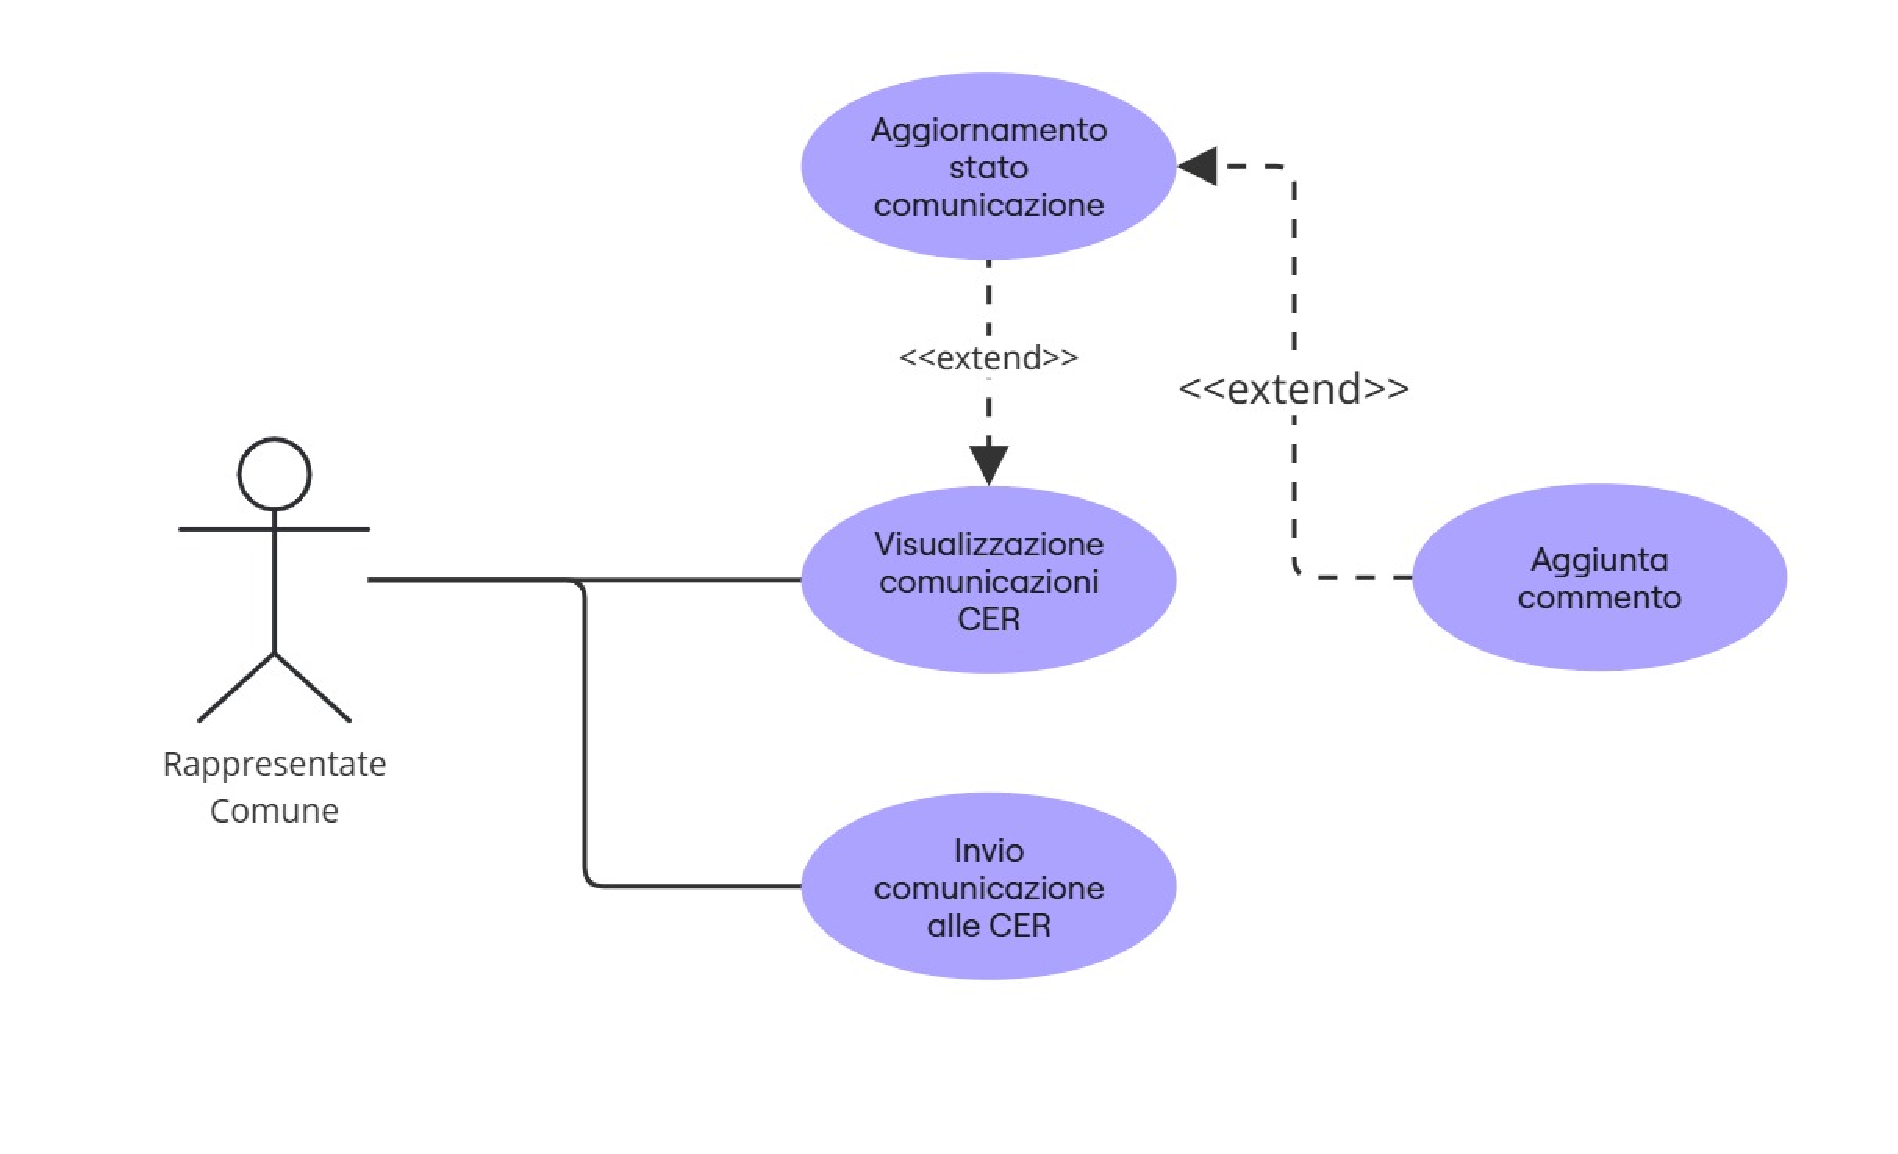
\includegraphics[width=0.9\textwidth]{images/use_case/ucd_06.pdf}
    \caption{UCD-06}
    \label{fig:ucd06}
\end{figure}

% =========================================================
\paragraph*{Use Case RF-13: Gestione richieste di approvazione o supporto (Rappresentante del Comune)}
\subparagraph*{Riassunto:}
Questo use case descrive come il rappresentante visualizza e gestisce le richieste e comunicazioni inviate dalle CER che necessitano supervisione.

\subparagraph*{Descrizione:}
\begin{enumerate}
    \item Il rappresentante accede all’elenco richieste (nuove comunità da validare, segnalazioni tecniche/amministrative) dall'homepage dedicata al Comune.
    \item Seleziona una richiesta per visualizzarne i dettagli e la documentazione allegata.
    \item Aggiorna lo stato della richiesta (es. in lavorazione, approvata, respinta) dal menù a tendina e aggiunge un commento visibile agli amministratori della CER scrivendo nell'apposita area.
    \item Il sistema invia notifiche agli interessati e registra le azioni svolte.
\end{enumerate}

\subparagraph*{Eccezioni:}
\begin{itemize}
    \item Se la richiesta manca di informazioni, il rappresentante può richiedere integrazioni prima di decidere.
    \item Se la decisione richiede verifiche esterne, lo stato può essere temporaneamente sospeso.
\end{itemize}

% =========================================================
\paragraph*{Use Case RF-14: Comunicazioni istituzionali (Rappresentante del Comune)}
\subparagraph*{Riassunto:}
Questo use case descrive come il rappresentante invia comunicazioni o avvisi alle CER del territorio.

\subparagraph*{Descrizione:}
\begin{enumerate}
    \item Il rappresentante apre la sezione ``Comunicazioni'' dall'homepage dedicata al Comune e compone un messaggio includendo testo e allegati (PDF, immagini).
    \item Seleziona le CER destinatarie (tutte o subset) e invia la comunicazione.
    \item Il sistema recapita i messaggi nelle aree notifiche delle CER e invia opzionalmente email.
    \item Le comunicazioni vengono registrate e disponibili per consultazione futura.
\end{enumerate}

\subparagraph*{Eccezioni:}
\begin{itemize}
    \item Se gli allegati superano il limite di dimensione, il sistema blocca l’invio e richiede riduzione.
    \item Se alcuni destinatari non sono raggiungibili, il sistema notifica l’errore e fornisce la lista parziale di recapito.
\end{itemize}
% =========================================================
\subsection*{Use Case Diagram – Requisiti funzionali per i Membri della CER}
% =========================================================

% ------------------------
\paragraph*{UCD-07 – Visualizzazione e confronto}
\begin{itemize}
    \item RF-15 – Visualizzazione dati energetici personali
    \item RF-16 – Confronto con la comunità
\end{itemize}

\begin{figure}[H]
    \centering
    
\includegraphics[width=0.9\textwidth]{images/use_case/ucd_07.pdf}
    \caption{UCD-07}
    \label{fig:ucd07}
\end{figure}

% =========================================================
\paragraph*{Use Case RF-15: Visualizzazione dati energetici personali (Membro CER)}
\subparagraph*{Riassunto:}
Questo use case descrive come un membro della CER visualizza i propri dati energetici personali.

\subparagraph*{Descrizione:}
\begin{enumerate}
    \item Il membro accede all’area personale e seleziona ``I miei dati energetici''.
    \item Il sistema mostra consumo, quota di energia condivisa, produzione (se prosumer) e trend temporali tramite grafici e valori numerici.
    \item I dati possono essere aggiornati periodicamente o in tempo reale se disponibile il feed.
    \item L’utente può esportare o salvare viste specifiche tramite le opzioni ``Salva'' ed ``Esporta''.
\end{enumerate}

\subparagraph*{Eccezioni:}
\begin{itemize}
    \item Se il feed dati non è aggiornato, il sistema mostra l’ultima rilevazione valida e un avviso di staleness.
    \item Se manca l’associazione tra utente e smart meter, il sistema indica il problema.
\end{itemize}

\subparagraph*{Estensioni:}
\begin{itemize}
    \item Avvisi personalizzabili (es. soglie consumo).
\end{itemize}

% =========================================================
\paragraph*{Use Case RF-16: Confronto con la comunità (Membro CER)}
\subparagraph*{Riassunto:}
Questo use case descrive come un membro confronta i propri consumi/produzione con la media della comunità in forma anonima.

\subparagraph*{Descrizione:}
\begin{enumerate}
    \item Il membro seleziona la funzione ``Confronta con la comunità'' dall'area personale.
    \item Il sistema aggrega i dati della comunità (anonimizzati) di cui l'utente è membro e calcola medie e percentili per il periodo selezionato.
    \item Viene mostrato un grafico comparativo o tabella riassuntiva che evidenzia la posizione del membro rispetto alla media.
    \item L’utente può filtrare per periodo, tipologia di consumo e visualizzare suggerimenti per migliorare l’efficienza.
\end{enumerate}

\subparagraph*{Eccezioni:}
\begin{itemize}
    \item Se i dati aggregati non sono sufficienti per preservare l’anonimato (troppi pochi membri), il sistema non mostra i confronti e informa l’utente.
    \item Se i dati comunitari sono incompleti, il sistema mostra risultati parziali.
\end{itemize}

% =========================================================
\paragraph*{UCD-08 – Notifiche e segnalazioni}
\begin{itemize}
    \item RF-17 – Notifiche e avvisi
    \item RF-18 – Partecipazione e segnalazioni
\end{itemize}

\begin{figure}[H]
    \centering
    
\includegraphics[width=0.9\textwidth]{images/use_case/ucd_08.pdf}
    \caption{UCD-08}
    \label{fig:ucd08}
\end{figure}

% =========================================================
\paragraph*{Use Case RF-17: Notifiche e avvisi (Membro CER)}
\subparagraph*{Riassunto:}
Questo use case descrive come il sistema notifica ai membri eventi rilevanti e come i membri consultano le notifiche.

\subparagraph*{Descrizione:}
\begin{enumerate}
    \item Il sistema genera notifiche per eventi come aggiunta di nuovo impianto, approvazione richiesta, anomalie dati.
    \item Le notifiche vengono mostrate nell’area personale con un contatore di elementi non letti.
    \item Il membro può aprire ogni notifica per vedere dettagli e allegati, e marcarla come letta.
    \item Le notifiche importanti possono essere inviate anche via email o SMS se abilitato.
\end{enumerate}

\subparagraph*{Eccezioni:}
\begin{itemize}
    \item Se l’invio di email/SMS fallisce, il sistema mantiene la notifica interna e registra l’errore.
    \item Se il membro disabilita notifiche via email/SMS, il sistema non invia comunicazioni esterne.
\end{itemize}

\subparagraph*{Estensioni:}
\begin{itemize}
    \item Filtri e preferenze per scegliere quali tipologie di notifiche ricevere.
\end{itemize}

% =========================================================
\paragraph*{Use Case RF-18: Partecipazione e segnalazioni (Membro CER)}
\subparagraph*{Riassunto:}
Questo use case descrive come i membri inviano segnalazioni o richieste di supporto all’amministratore o al rappresentante del Comune.

\subparagraph*{Descrizione:}
\begin{enumerate}
    \item Il membro accede alla sezione ``Segnalazioni / Supporto'' e compila un modulo con titolo, descrizione, destinatari e allegati (foto, PDF).
    \item Il sistema crea la segnalazione, assegna uno stato iniziale (es. inviata) e genera un ticket con identificativo.
    \item L’amministratore o rappresentante consulta la segnalazione, assegna responsabile e aggiorna lo stato (presa in carico, risolta).
    \item Il membro può seguire lo stato della segnalazione e ricevere notifiche sugli aggiornamenti.
\end{enumerate}

\subparagraph*{Eccezioni:}
\begin{itemize}
    \item Se il modulo è incompleto, il sistema segnala gli errori e impedisce l’invio.
    \item Se gli allegati superano i limiti consentiti, l’invio viene bloccato.
\end{itemize}
